\section{Artefact}\label{sec:artefact}
This section describes the created NetLogo model named `FoodDelivery'.

The world that is being modelled is what is known as, the last mile in the food delivery industry.
This term is used for the last step in the delivery of online ordered goods.

Companies in the food delivery industry offer a service to three parties:
\begin{itemize}
    \item restaurants: they sell its food in a portal made by the delivery company.
    \item consumers: they buy food from a restaurant using the same portal.
    \item deliverers: they are steered by a mobile app also from the delivery company.
\end{itemize}

The steps in the food ordering and delivery proces are:
\begin{itemize}
    \item When a customer orders a meal, a message is sent to the restaurant.
    \item The restaurant starts preparing the meal, this may take some time (say on average 10 minutes).
    \item When it starts preparing, a deliverer is needed.
    \item A deliverer can claim the delivery (or is assigned) and starts cycling towards the restaurant.
    \item When the deliverer arrives at the restaurant it may have to wait until the meal is ready.
    \item When the meal is ready the deliverer takes it and start driving towards the customer.
    \item It may happen that no deliverer claims the meal, or it takes to long for the deliverer to get to the restaurant,
then the meal will be thrown away.
    \item If the meal gets delivered, the customer is happy
    \item If the meal is not delivered, the customer is unhappy.
    \item If a customer is unhappy it will eventually stop ordering meals.
\end{itemize}

This all takes place in a city with restaurants and customers.
The deliverers have to cycle to the restaurant and then to the customer.
The best route will be provided by the app the deliverers use.

The money for the delivery company is earned by charging the restaurants per delivery.
The companies interest is thus to have as many deliveries as possible.
This means they want to have happy customers and enough deliverers to keep them happy.

This is more or less how the process works in the real world.

\subsection{Conceptional model}\label{subsec:conceptional-model}
The FoodDelivery model has the same types of agents:
-deliverers \\
-restaurants \\
-customers \\

The delivery company itself is not modelled explicitly, they are what is called the observer.

\paragraph{Customers} will order food from a restaurant.
Orders are not equally distributed per day, peek hours are: breakfast, lunch and diner.
They will on average order once a week.
The restaurant is selected at random.
In the model the probability distribution shown in figure~\ref{fig:food_ordering_distribution} is used.
If a meal is not delivered the customer is not satisfied and their satisfaction level is subtracted 1 point
Customers stop ordering food if they have a satisfaction level below -1.

\begin{figure}
    \centering
    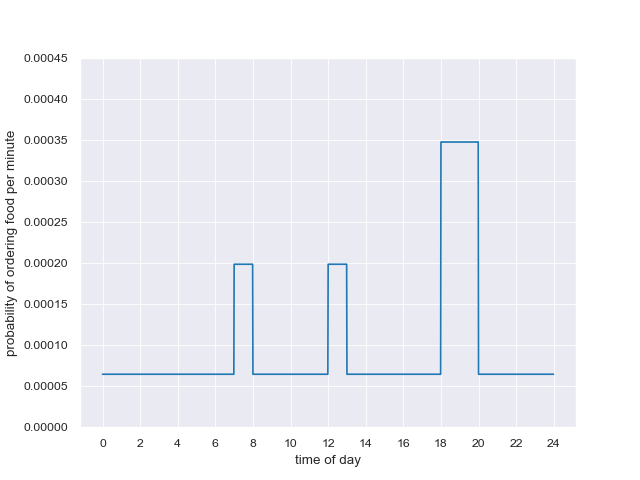
\includegraphics[width=8.5cm]{sections/pics/food_ordering_distribution}
    \caption{Food ordering probablities for one day}
    \label{fig:food_ordering_distribution}
\end{figure}

\paragraph{Restaurants} accept any order, and are open all the time.
When an order arrives, the preparation starts.
This preparation-time is Gaussian distributed, the mean and standard deviation can be set.
Upon order arrival the meal can be assigned to a deliverer.
When the meal is ready it can be picket up for a waiting time that can be set.
After this waiting time the meal will be thrown away.

Not in the current model, but what could be interesting are:
-restaurants cannot leave the system if they have not enough orders\\
-the freshness of the meal is not taken into account\\

\paragraph{Deliverers} are the only agents that can move.
There are 2 possibles meals distribution strategies that can be set:
-distribute meals equally among the deliverers\\
-assign a meal to the closest free deliverer\\

When a meal is assigned to the deliverer it will take the shortest route
to the restaurant, wait until the meal is ready and move to the customer.
The deliverer will lose its assigned meal if he/she does not arrive before the waiting time is over.

As a design choice deliverers have no shifts, they work all the time.
Using shifts would make the model much more complicated, this could be done in a next version.

\paragraph{The world} consists op a grid of squares, some squares will be blocks of buildings and others represent the streets.
On this grid restaurants and customers are placed at random on the building blocks.
The delivers are at the start randomly placed on the streets, they can only move on the street patches.

The goal of the delivery company is not the profit instead of this their goal is to have as many deliveries as possible

\subsection{Computer model}\label{subsec:computer-model}
The world is for a large part build using the code from the Taxi Cab model.
The streets, how the delivers move is from their model, only the traffic lights where removed.

The design of the grid is show in figure~\ref{fig:grid} and figure~\ref{fig:grid closeup}
\begin{figure}
    \centering
    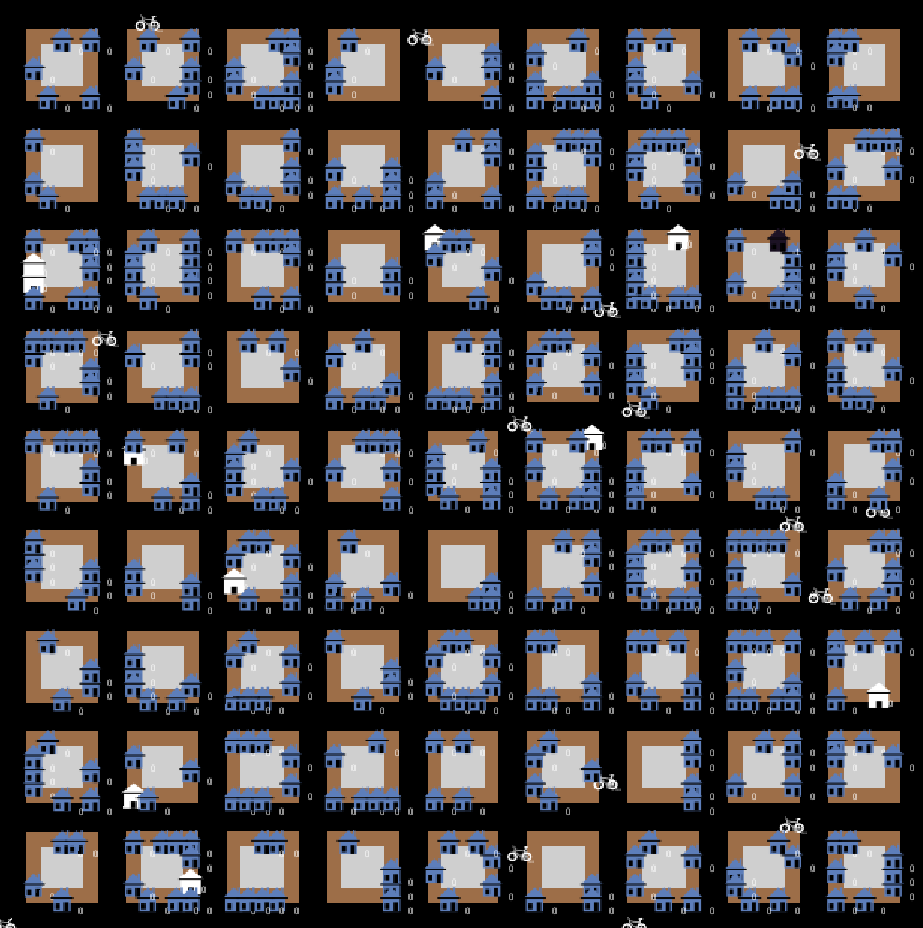
\includegraphics[width=8.5cm]{sections/pics/grid}
    \caption{Fooddelivery grid}
    \label{fig:grid}
\end{figure}
\begin{figure}
    \centering
    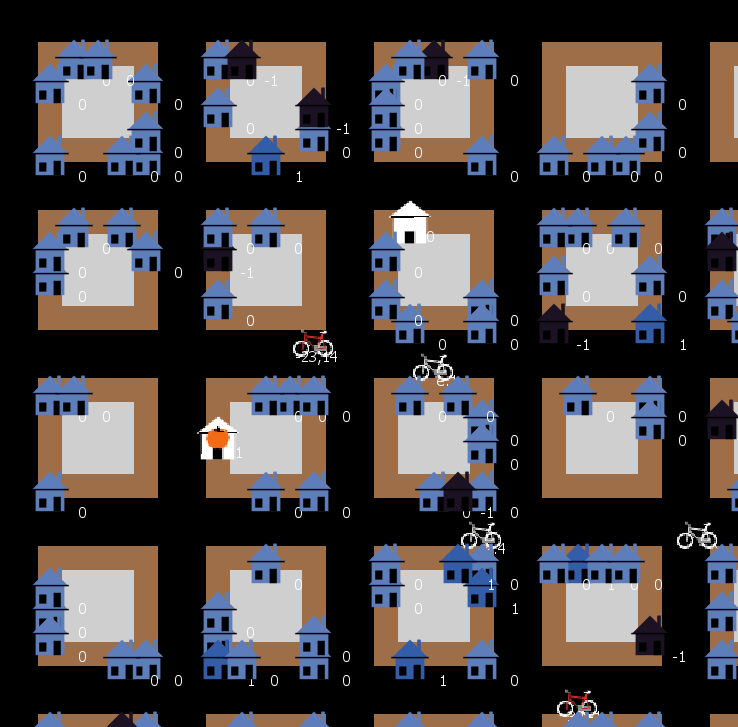
\includegraphics[width=8.5cm]{sections/pics/grid_closeup}
    \caption{Fooddelivery grid closeup}
    \label{fig:grid closeup}
\end{figure}
The agents can be seen in figure~\ref{fig:agents}.
\begin{figure}
     \centering
     \begin{subfigure}[m]{0.1\textwidth}
         \centering
         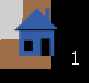
\includegraphics[width=\textwidth]{sections/pics/cust_happy}
         \caption{Customer with happyness score}
     \end{subfigure}
     \hfill
     \begin{subfigure}[m]{0.1\textwidth}
         \centering
         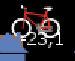
\includegraphics[width=\textwidth]{sections/pics/del_on_its_way}
         \caption{Deliverer on route to loc 23,1}
     \end{subfigure}
     \hfill
     \begin{subfigure}[m]{0.1\textwidth}
         \centering
         
\includegraphics[width=\textwidth]{sections/pics/meal_prep}
         \caption{Restaurant with meal ordered on top and number of ordered}
     \end{subfigure}
      \hfill
     \begin{subfigure}[m]{0.1\textwidth}
         \centering
         
\includegraphics[width=\textwidth]{sections/pics/meal_ready}
         \caption{Restaurant with meal ready on top and number of ordered}
     \end{subfigure}
        \caption{Agents examples}
        \label{fig:agents}
\end{figure}

In NetLogo, everything works on ticks, during 1 tick all code in the go procedure is executed.
During programming the programmer must deside what to do in that tick.
This makes it difficult to program future behaviour.

The order of execution of agents of one kind is arbitrary.

The program is available inside a git repository available at GitHub~\footnote{\url{https://github.com/evertvankammen/FooddeliveryNetlogo}}
This repository also contains the Python code to automate running the model with different parameters.

\section{Results of simulations}\label{sec:results-of-simulations}
Consumers order meals from restaurants they like, if a meal is delivered cold they dislike the restaurant.
If they dont like the restaurant they will not place any orders anymore at that restaurant.

Restaurants create meals, if they dont get any orders for some time they quit.

The delivery provider make money for each order placed via their system, at the end they must have enough deliverers so that
customers keep ordering.
They have to pay the deliverers for the deliveries.



\subsection{Model variant 1}
Here come the results belonging to variant where deliverers are hired and paid an hourly wage.
The company destributes deliveries equally among the hired employees.
The company has to deside on how many to hire and for which periods.


\subsection{Model variant 2}
Here come the results where deliverers are independent contractors.
Deliverers come and go whenever they are pleased, like a open market.
Now deliverers have to deside to become a deliverer, deside to stop and to decide to go for a delivery.
To keep this simple, the meals are destributed among the available deliverers.
If a delivery person does not make enough many during a day they will quit.
